\chapter{Leveransetest}
\textit{Leveransetesten ble gjennomført sammen med PO-Veileder 06.06.2018.}
\section{\textbf{Struktur av leveransetest}}
\newthought{Vi strukturerte leveransetesten} på den måten at den fungerte som en sjekkliste av all funksjonalitet vi laget i løsningen, og fargekodet hver kategori. Hvert punkt i testen består av et funksjonelt spørsmål med ja/nei (bestått eller ikke bestått)  og et felt for kommentarer.

Før vi gikk gjennom leveransetesten forberedte vi et eget bord med løsningen klar til veileder med testen printet ut. Deretter gikk vi gjennom hvordan testen er strukturert og hvordan den skulle gjennomføres.

Vi fikk kommentarer om at fargevalg på innloggingssiden kunne vært bedre og valgte å rette opp i dette før leveranse. I tillegg påpekte veileder at søkefunksjon på beholdningsiden burde vise resultater på tvers av kategorier, og vi valgte derfor å legge dette i product backlog til fremtidige sprinter.
  
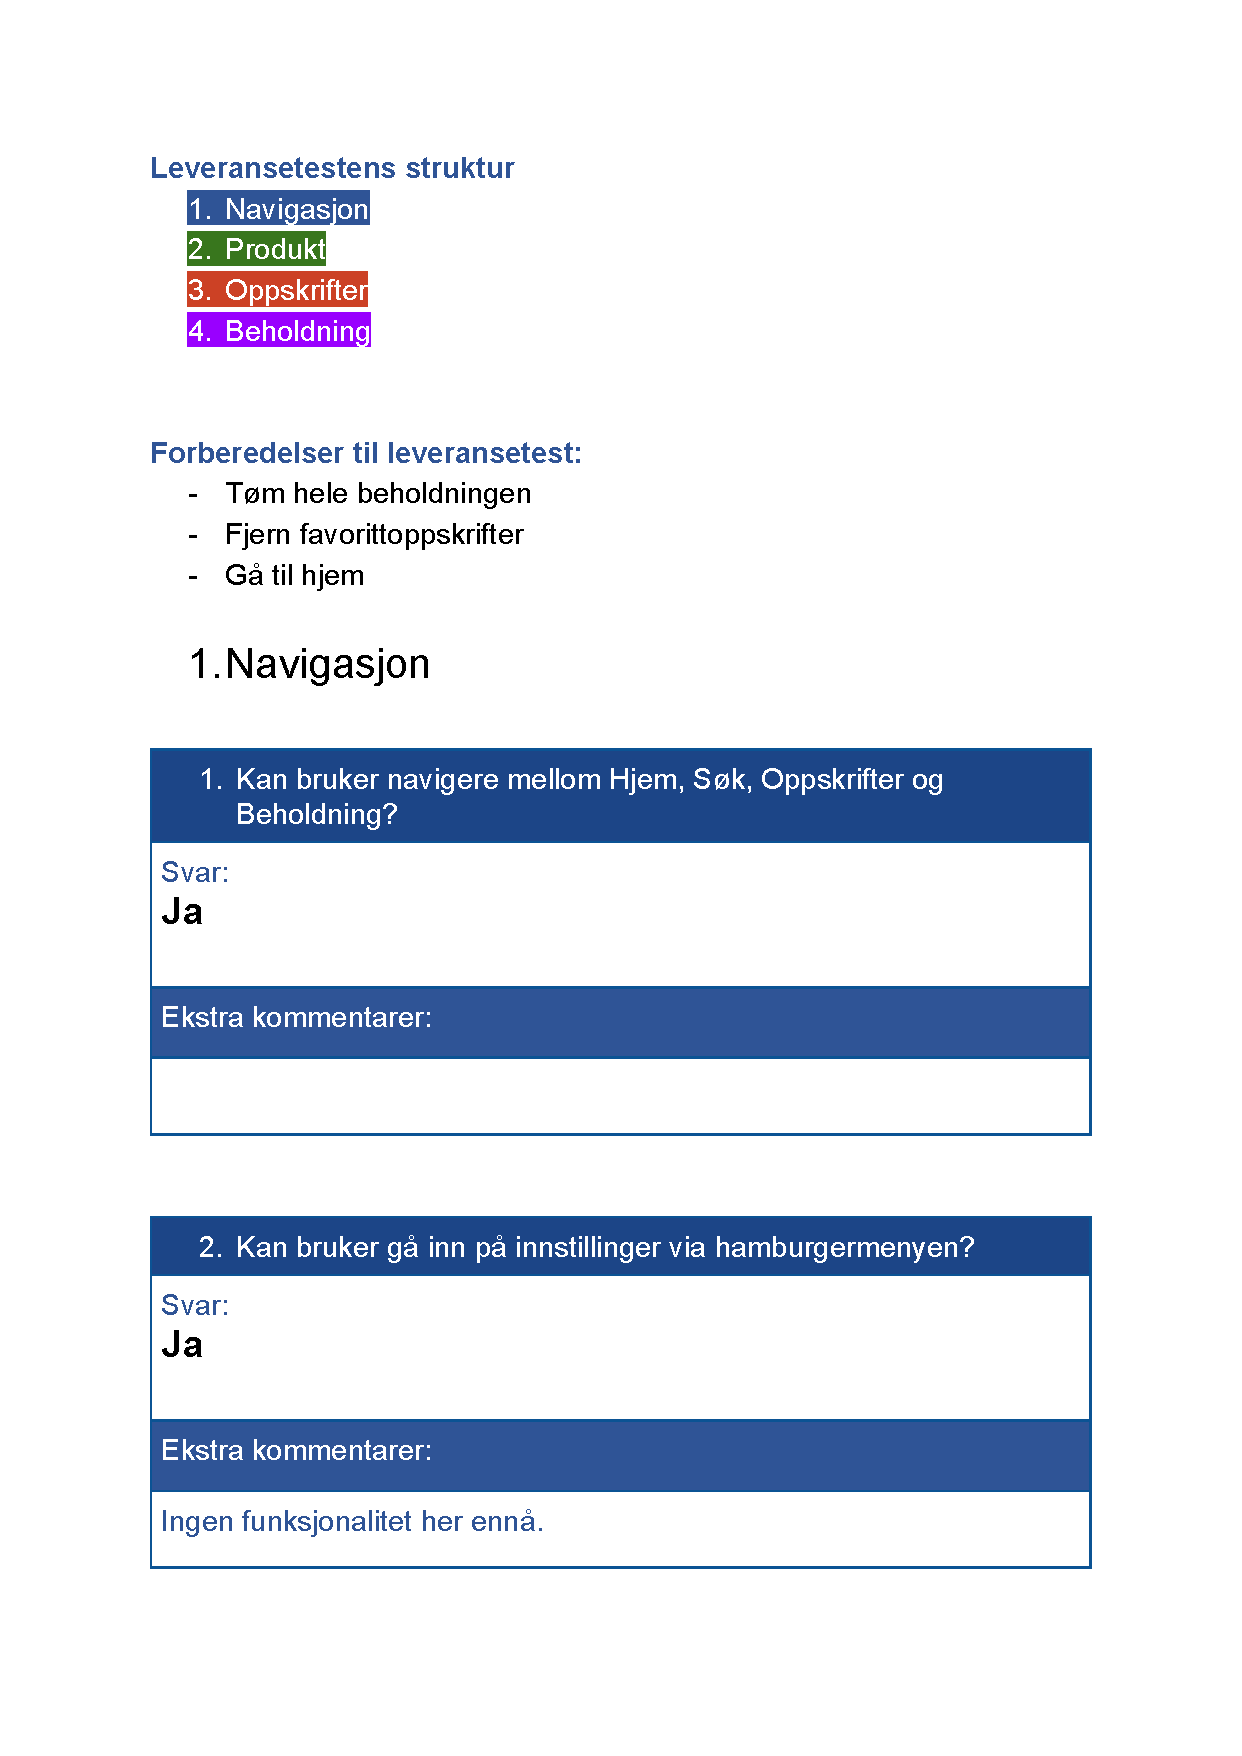
\includepdf[pages=-]{figures/vedlegg/Leveransetest}